%%===============================================================
%%===============================================================
\chapter{Development Process}
%%===============================================================
%%===============================================================

This chapter outlines a development method know as Test Driven Development (TDD). TDD insures thorough testing of code throughout its development and implementation life cycle, resulting in improved reliability. Coupled with the process of Refactoring, TDD produces robust code that is easily read and understood. Concepts of TDD and Refactoring shall be briefly explained in the following sections. It is recommended that OpenFCST developers use this approach when developing new classes.

%%===============================================================
\section{Test Driven Development}
%%===============================================================
    
Test Driven Development (TDD) is a software development methodology which is rather different compared to the typical development process generally acquired when learning programming. Imagine a programmer is given a problem for which they must provide a software solution. Instead of diving in ``head first`` and writing code to provide the solution, a TDD programmer first writes a number of Unit tests. Unit testing is a method by which individual units of source code are tested to determine if they are fit for use. In object oriented programming units are individual member functions.  The Unit tests define acceptable behavior of the code that the programmer intends to create. Once the Unit tests have been created, the programmer may then write the actual code that will provide their programming solution. Whilst writing this code the programmer uses their Unit tests to ensure the written code behaves correctly,i.e. passes the test.
     
A more detailed description of the TDD methodology as seen in Figure \ref{fig:TDD1}:

\begin{figure}[h]
\centering
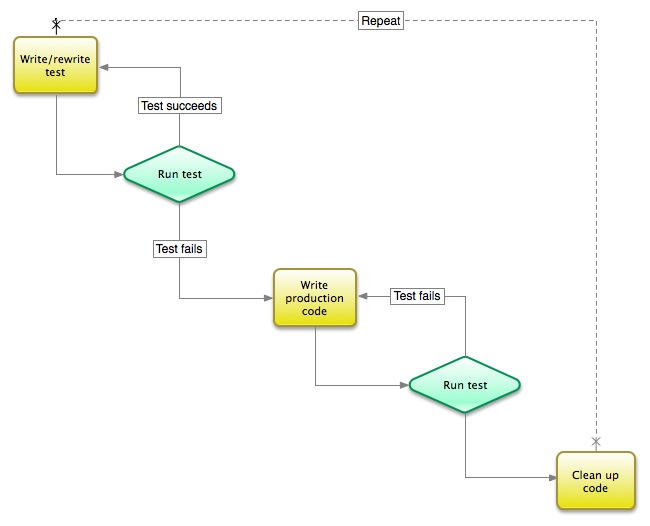
\includegraphics[width=0.9\textwidth]{figures/tdd-diagram-3.jpeg}
\caption{\label{fig:TDD1} TDD Cycle.}
\end{figure} 
     
\begin{enumerate}
\item Creation of a set of Unit tests that define the correct behavior of production code. Note: We must ensure that these tests initially fail. 
\item Creation of production code and subsequent checks to see if it passes  unit tests. Work on production code continues until all tests are passed.
\item Code is cleaned. Refactoring to increase readability and understanding of code.
\item More test cases may be added in order to ensure sufficient testing. The number of unit tests required for satisfactory testing is subject to the programmers judgment.
\end{enumerate}
     
\textbf{ Advantages of TDD are as follows:}
\begin{enumerate}
\item Increased reliability of code.
\item Programmers who write more tests are more productive.
\item Not just a validation of correctness: TDD also drives development by forcing the programmer to think strongly about how their code will be used. This leads to smaller, more focused classes, and cleaner interfaces.
\item Unit tests act as documentation: Testing functions are understandable examples of how the production code should be used.
\item TDD ensures consistent testing off all resources throughout the development of a piece of software.
\end{enumerate}

\subsection{Unit Tests}
Unit tests, as already mentioned, are tests that determine if individual units of source code are fit for use. It is important that unit tests are written very simply in order to ensure correctness (since there is no tests to ensure that the unit tests are correct). The following is a simple example of a test function and the corresponding production code it is intended to test.
      
\textbf{Unit Test:}
\begin{lstlisting}
void testAdd(){
  
  int expectedAnswer = 5;
  int answer = add(3 ,2);
  
  TEST_ASSERT(expectedAnswer == answer); //Check to see if output is as expected, and make record if it is not.
  
}
      
\end{lstlisting}
      
      \textbf{Production code (under test):}
      \begin{lstlisting}
int add(int a, int b){
  return a*b; //Obviously this will cause the test to fail
}
      \end{lstlisting}
      
      Obviously, the above test will fail because the function \emph{add()} has been implemented incorrectly. Using a Unit testing library such as CppTest we will recieve the following output:
      
      \begin{lstlisting}
FailTestSuite: 0/0, 0% correct in 0.000002 seconds
  Test:    testAdd
  Suite:   ExampleSuite
  File:    mytest.cpp
  Line:    9
  Message: "expectedAnswer == answer"
      \end{lstlisting}

%%================
\subsection{TDD Implementation in the OpenFCST}  
The unit testing structure that is implemented in OpenFCST is built using a library called CppTest.  CppTest is a portable, powerful, and simple unit testing framework for handling automated tests in C++. The focus lies on usability and extendability.

Several output formats, including simple text output, compiler-like output, and HTML can be produced. The tests suit is launched from the system builder class's \texttt{run\_tests()} function, see Figure \ref{fcstUnit}. Firstly, unit tests are run (which will test individual components of various classes), then system level tests. 
      
\FloatBarrier
\begin{figure}[h]
\begin{center}
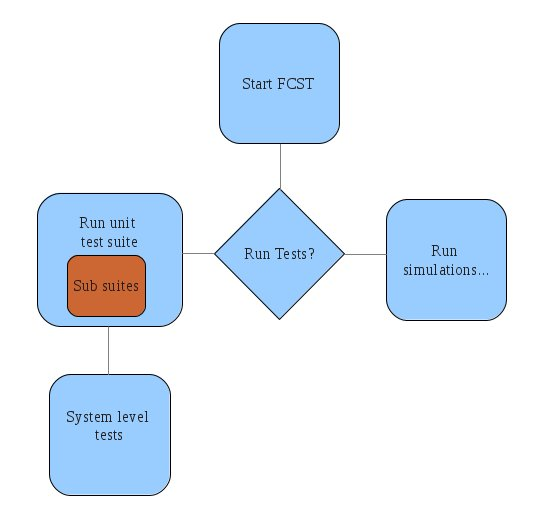
\includegraphics[width=0.7\textwidth]{figures/FCST_TDD.jpeg}
\caption{\label{fcstUnit} TDD illustration scheme.}
\end{center}
\end{figure}
\FloatBarrier

The operation is as follows.

The ``Run tests'' parameter is set in the main parameter file.

\begin{center}
\begin{lstlisting}
  set Run tests = true
\end{lstlisting}
\end{center}

The run test function in SimulatorBuilder is called, which in turn calls the OpenFCST testing suite.

\begin{center}
  \begin{lstlisting}
    void SimulatorBuilder<dim>::run_test()
    {	
	deallog << "==================Running Unit Tests===================" << std::endl;

	FcstTestSuite::run_tests();
	
	deallog << "================System Tests Complete==================" << std::endl;
  \end{lstlisting}
\end{center}

The OpenFCST test suite runs all of the unit testing suites that it is composed of (currently only the OpenFCST units testing suite)
\begin{center}
\begin{lstlisting}
bool FcstTestSuite::run_tests()
{
  Test::Suite ts;

  //add sub tests suites
  ts.add(std::auto_ptr<Test::Suite>(new FcstsUnitsTestSuite));
  ts.add(std::auto_ptr<Test::Suite>(new IonomerAgglomerate3Test));		

  Test::TextOutput output(Test::TextOutput::Verbose);
  return ts.run(output);

} 
\end{lstlisting}
\end{center}
Below is an example of an individual ''sub-testing'' suite. Each individual unit test is added to the test suite in the constructor and will be called individually when the .run() function is called.
\begin{center}
\begin{lstlisting}
#ifndef _FCST_UNITS_TESTSUITE
#define _FCST_UNITS_TESTSUITE

#include <cpptest.h>
#include "fcst_units.h"



class FcstsUnitsTestSuite: public Test::Suite
{
  public:
      FcstsUnitsTestSuite()
      {
	//Add a number of tests that will be called during Test::Suite.run()
	//Generic cases
	TEST_ADD(FcstsUnitsTestSuite::perBigToSmallTest);
	TEST_ADD(FcstsUnitsTestSuite::bigToSmallTest);
	TEST_ADD(FcstsUnitsTestSuite::perSmallToBig);
	TEST_ADD(FcstsUnitsTestSuite::smallToBig);
	  
	  //specific Cases
	TEST_ADD(FcstsUnitsTestSuite::btuToKwh);
	TEST_ADD(FcstsUnitsTestSuite::kwhToBtu);
      }
  protected:
      virtual void setup()     {} // setup resources... called before Test::Suite.run()
      virtual void tear_down() {} // remove resources...called after Test::Suite.run()    
      
  private:
	  //Generic cases
      void perBigToSmallTest();
      void bigToSmallTest();
      void perSmallToBig();
      void smallToBig();
      
      //Specific cases
      void btuToKwh();
      void kwhToBtu();
}; 

#endif
\end{lstlisting}
\end{center}

Below is an example of an individual unit test taken from the ``FcstsUnitsTestSuite'' test suite. It checks that the function \texttt{convert} correctly converts units of BTU to units of KJ.
\begin{center}
\begin{lstlisting}
void FcstsUnitsTestSuite::btuToKwh()
{
  TEST_ASSERT(Units::convert(1,Units::BTU_to_KJ) == 1.054);

}
\end{lstlisting}
\end{center}

%%================
\subsection{Implementing a new test suite}

If you would like to add a unit test suite for a class that you are creating, follow these steps:

\begin{enumerate}
 \item Create the class\_test.h and class\_test.cc files in the unit\_test folders (use the existing .h and .cc files as templates).
 \item Add an include statement to your new class\_test.h file in FCST\_TEST\_SUITE.h (under code comment "List of sub suites").
 \item In FCST\_TEST\_SUITE.cc, add your new test class in the run\_tests() function.
\end{enumerate}

If you would like your test to be able to see private variables inside the class that it is testing, you must add it as a friend to that class:
\begin{enumerate}
 \item Go to the header of the class you are testing (class.h).
 \item At the top of  the file (outside namespace scope), make a reference to your test class (e.g. "class nameOfTestClass;").
 \item In the class's declaration, write the friend statement above the public section (e.g. "friend class ::nameOfTestClass;").
\end{enumerate}

%%================    
\subsection{Refactoring}
Refactoring is a technique for restructuring existing code to improve it's readability and user understanding, without changing the behaviour of the code in any way. When refactoring code, a programmer looks for ``Bad Programming Smells'' and uses various methods to remove them. Code smells are not bugs, but weakness in code design that makes code difficult to understand and can lead to bugs being introduced into the code.
      
      Some examples of bad programming smells:
      \begin{enumerate}
       \item Duplicated code: identical or very similar code exists in more than one location.
       \item Long method: a method, function, or procedure that has grown too large or complicated.
       \item Inappropriate intimacy: a class that has dependencies on implementation details of another class.
       \item Too many parameters: a long list of parameters in a procedure or function make readability and code quality worse.
       \item Complex conditionals.
       \item Temporary variables and fields.
       \item Use of primatives rather than objects.
       \item Classes and functions with multiple responsibilities.
      \end{enumerate}

      The following is an example of code that exhibits bad smells (see if you can spot them):
      
      \begin{center}
      \begin{lstlisting}
void sendMessage(Message dataToSend, string phoneNumber, string networkOperator){
  
  string areaCode = "213";
  
  if (networkOperator == "Rogers"){
    string _phoneNumber = areaCode + "4" + phoneNumber;
    MessageBuffer b;

    for(int i=0; i < dataToSend.length(), i++)
      b.pack(dataToSend[i]);
    
    send(b, _phoneNumber)

  }
  else if(networkOperator == "Telus"){
  
    string _phoneNumber = areaCode + "9" + phoneNumber;
    MessageBuffer b;

    for(int i=0; i < dataToSend.length(), i++)
      b.pack(dataToSend[i]);
    
    send(b, _phoneNumber)
  
  }
}
      \end{lstlisting}
      \end{center}
      
      Bad smells include local data (the area codes should not be stored locally but should be the responsibility of another class such as PhoneBook), and duplicate code inside either if statement.
      The following code represents the above code refactored. The refactoring patterns extract method has been used to replace the code from within the for loop, the pattern extract data
      has been used to remove the local variables areaCode as well as the if statement comparisons. The result is code that is shorter, more easily understood, and more easily reused.
      
       \begin{center}
      \begin{lstlisting}
void sendMessage(Message dataToSend, string phoneNumber, string networkOperator){
  
  string fullPhoneNumer = PhoneBook::getAreaCode() + PhoneBook::getOperatorCode(networkOperator) + phoneNumber;
  MessageBuffer buffer = package(dataToSend);
  send(buffer, _phoneNumer)''
  
}

MessageBuffer package(Message dataToSend){
  MessageBuffer buffer
  
  for(int i=0; i < dataToSend.length(), i++)
    buffer.pack(dataToSend[i]);

  return buffer;
}
      \end{lstlisting}
      \end{center}
      
      Also note the change of variable names. The new names do a better job at describing their purpose.
      
%%================      
\subsection{Unit Standards}
OpenFCST uses centimetres, grams and seconds (CGS) units for most of its variables.

  
%%========================================================================================
%%========================================================================================